\section{Corner Cutting}
\label{sec:erm-corner-cutting}
Should finding the exact ridge be the goal --- rather than just the \sap{2} and a ridge estimate --- and the alternative tangent discussed above not be sufficient, multiple strategies can be envisioned, all of which aim at somehow reducing the perpendicular component of the spring force while avoiding or minimising the instabilities discussed above.

\subsubsection{What is corner cutting}
The spring force tries to keep each image as close as possible to its neighbours.
Without any further influence, the images would align evenly spaced in a straight line.
However, since there are other forces at work, perpendicular to the path, $\vF^\text{t}$, an equilibrium between the conflicting forces will be reached, when they are equal in length but with opposite direction,
\beq{corner-cutting-equilibrium}
\vF^{\text{S}\perp} = -\vF^\text{t},
\eeq
producing a systematic error which is commonly referred to as corner cutting as seen in \fref{fig:corner-cutting}.
Since the goal of the whole method is to fulfil \fref{eq:ridge-force}, such an equilibrium can be unsatisfactory.

This problem existed in the infancy of NEB calculations but was made a thing of the past with more numerically suitable tangent and spring force definitions~\cite{neb-tangent-2000}.
These changes are not directly applicable to ridge calculations due to intrinsic stability issues which are dampened by the perpendicular component of the spring force.
However, once the path is sufficiently well behaving and near the ridge, minimising the corner cutting could be done.

\begin{SCfigure}[5.0][h]
\centering
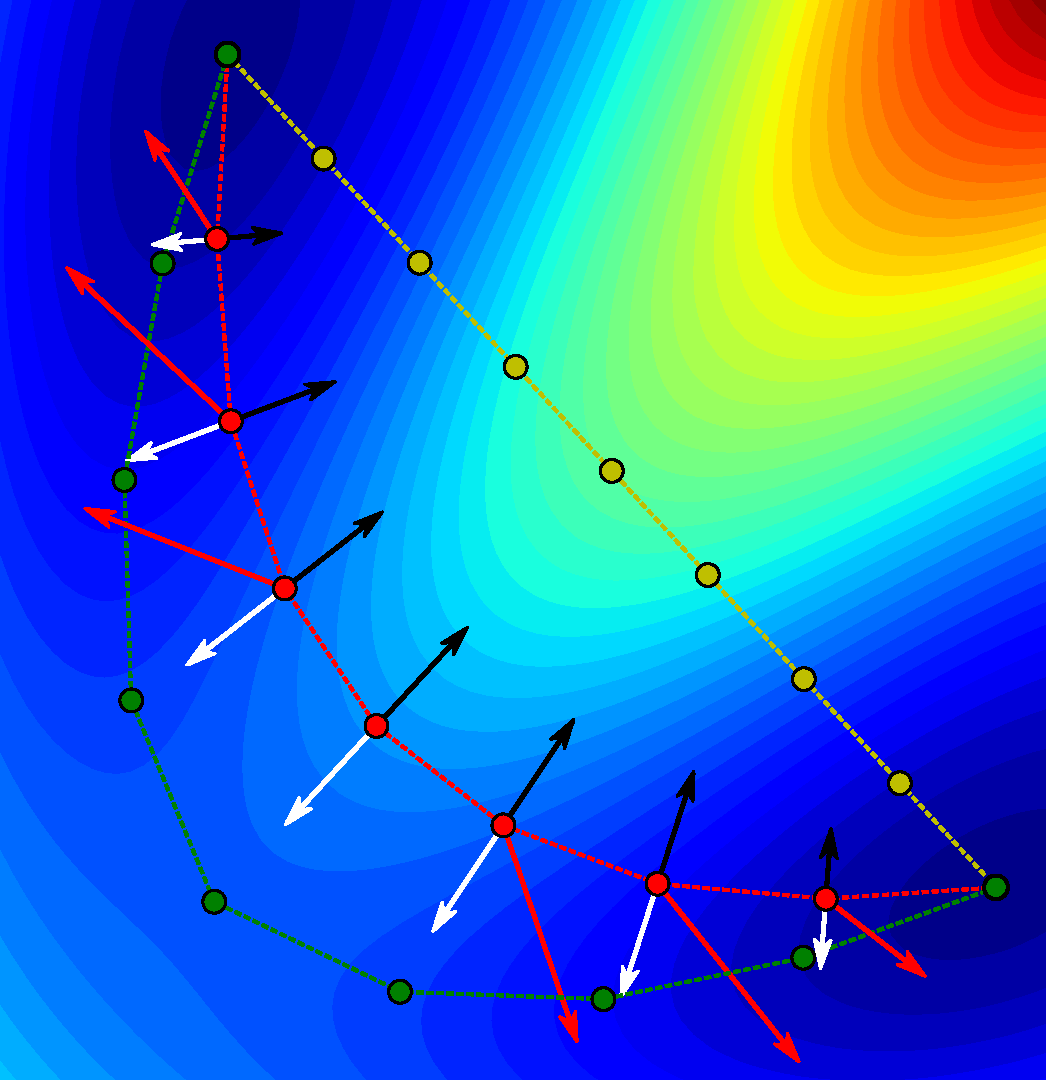
\includegraphics[width = 0.5\linewidth]{corner-cutting}
\caption{
An example of corner cutting.
The yellow path is the initial linear interpolation on which the spring forces are zero (since it is the shortest possible path) and the green path is the converged MEP without any perpendicular spring force components.
The red path has converged to an equilibrium between the perpendicular components of the spring force (black arrows) and PES force (white arrows).
The red arrows are the full PES force.
High potential areas are red and low potential areas are blue.
}
\label{fig:corner-cutting}
\end{SCfigure}

\subsection{Minimise corner cutting}
\textit{After publishing paper \ref{pap:second-order} some effort went into finding the exact ridge instead of paths that suffer from corner cutting.
The methods and ideas presented here serve more as a detailed outlook for future work than a complete study.}
\vspace{1em}

In order to reduce/remove corner cutting, the perpendicular component of the spring force must be removed/reduced at each image.
Then in tune with the equilibrium presented in \fref{eq:corner-cutting-equilibrium}, \fref{eq:ridge-force} will be fulfilled and the exact ridge found.

Using the dual tangent scheme, presented above, it is possible to significantly reduce the numerical instabilities of the ridge calculation.
In some test cases even allowing for the complete exclusion of the perpendicular spring force after turning on the climbing image.
However, should this not be possible, a multiplication factor, $\xi_i \in [0, 1)$, for the perpendicular spring force,
\beq{spring-force-perpendicular}
\vF_i^{\text{S}\perp} = \vF_i^\text{S} - (\vF_i^\text{S} \cdot \uvt_i)\uvt_i,
\eeq
can be defined,
\beq{spring-force-reduction}
\vF_i^{\text{S, eff.}\perp} = \xi_i \vF_i^{\text{S}, \perp},
\eeq
to iteratively bring the effective perpendicular component, $\vF_i^{\text{S, eff.}\perp}$, to zero and thus converging to the exact ridge.

Multiple schemes for reducing $\xi_i$ can be envisioned.
One, that initial testing showed to be successful, is reducing $\xi_i$ each time corner cutting is detected and then continuing the iterative convergence until either corner cutting is detected again or the path is fully converged to the ridge.
By how much $\xi_i$ is reduced each time, could either be a fixed ratio or, preferably, dependant on the amount of corner cutting.\footnote{Only the fixed ratio scheme was tested.}
In order for the path to converge evenly, $\xi_i$ must be restricted to be of a similar magnitude as $\xi_{i-1}$ and $\xi_{i+1}$.
Using a scheme such as this, the corner cutting was significantly reduced in the test systems %\footnote{Both custom potentials and the Al self diffusion (\fref{chap:al}) systems were tested but not extensively.}
it was applied to.

It warrants repeating that the ridge method, as presented originally in paper \ref{pap:second-order}, is able to find the \sap{2} exactly without problem but if the ridge is curved, corner cutting will take place, except near the \sap{2}.
While the removal of corner cutting would present a truer picture of the ridge, the method as it stood is still of good use.
